%% LyX 2.1.3 created this file.  For more info, see http://www.lyx.org/.
%% Do not edit unless you really know what you are doing.
\documentclass[
12pt,
ngerman,
%american,
pointlessnumbers,
abstracton
]{scrreprt}


%-------------------------------------------------------------
% Packages
%-------------------------------------------------------------
\usepackage[
	automark,								 	% Kapitel in Kopfzeile
	headsepline,								% Trennlinie unter Kopfzeile
	ilines										% Trennlinie linksbündig ausrichten
]{scrpage2}


\renewcommand{\familydefault}{\sfdefault}
\usepackage[T1]{fontenc}
%\usepackage[ngerman]{babel}
%\usepackage[ansinew]{inputenc}
%\usepackage[T1]{fontenc}
\usepackage[latin1]{inputenc}
%\usepackage[utf8]{inputenc}
\usepackage{geometry}
\usepackage[acronym,toc,automake]{glossaries}
\geometry{verbose,tmargin=2.5cm,bmargin=3.5cm}
\pagestyle{plain}
\setlength{\parskip}{\medskipamount}
\setlength{\parindent}{0pt}
\usepackage{color}
\usepackage{babel}
\usepackage{array}
\usepackage{varioref}
\usepackage{textcomp}
\usepackage{multirow}
\usepackage{amsfonts}
\usepackage{amsthm}
\usepackage{amsmath}
\usepackage{graphicx}
\usepackage{setspace}
\usepackage{nomencl}
% the following is useful when we have the old nomencl.sty package
\providecommand{\printnomenclature}{\printglossary}
\providecommand{\makenomenclature}{\makeglossary}
\makenomenclature
\setstretch{1.2}

\makeatletter

%%%%%%%%%%%%%%%%%%%%%%%%%%%%%% LyX specific LaTeX commands.
%% Because html converters don't know tabularnewline
\providecommand{\tabularnewline}{\\}

%%%%%%%%%%%%%%%%%%%%%%%%%%%%%% User specified LaTeX commands.
% verschieden Symbole, Zeichen wie (c), ¤
\usepackage{textcomp,units}

% Mehr Platz zwischen Tabelle und Untertitel
\usepackage{caption}
\captionsetup[table]{skip=10pt}

%Kapitelzahl sehr groß
\makeatletter% siehe De-TeX-FAQ 
 \renewcommand*{\chapterformat}{% 
   \begingroup% damit \unitlength-Änderung lokal bleibt 
     \setlength{\unitlength}{1mm}% 
     \begin{picture}(10,10)(0,5) 
       \setlength{\fboxsep}{0pt} 
       %\put(0,0){\framebox(20,40){}}% 
       %\put(0,20){\makebox(20,20){\rule{20\unitlength}{20\unitlength}}}% 
       \put(10,15){\line(1,0){\dimexpr 
           \textwidth-20\unitlength\relax\@gobble}}% 
       \put(0,0){\makebox(10,20)[r]{% 
           \fontsize{28\unitlength}{28\unitlength}\selectfont\thechapter 
           \kern-.05em% Ziffer in der Zeichenzelle nach rechts schieben 
         }}% 
       \put(10,15){\makebox(\dimexpr 
           \textwidth-20\unitlength\relax\@gobble,\ht\strutbox\@gobble)[l]{% 
             \ \normalsize\color{black}\chapapp~\thechapter\autodot 
           }}% 
     \end{picture} % <-- Leerzeichen ist hier beabsichtigt! 
   \endgroup 
}

\usepackage{ %a4wide,
            ellipsis, fixltx2e, mparhack,   %Fehlerkorrektur für Marginalien
            booktabs, longtable             %schönere Tabellen
}  

%\usepackage[automark]{scrpage2}
%\automark[chapter]{chapter}
%\clearscrheadfoot
%\ohead{\\\headmark}
%\ihead{\includegraphics[scale=0.15]{logo.jpg}}%\pagemark}
%\ofoot[\pagemark]{\pagemark}


%Kurzfassung und Abstract (englisch) auf eine Seite
\renewenvironment{abstract}{
    \@beginparpenalty\@lowpenalty
      \begin{center}
        \normalfont\sectfont\nobreak\abstractname
        \@endparpenalty\@M
      \end{center}
}{
    \par
}



% schönerer Blocksatz!!
\usepackage{microtype}

\usepackage{ifpdf} % part of the hyperref bundle
\ifpdf % if pdflatex is used

%set fonts for nicer pdf view
 \IfFileExists{lmodern.sty}{\usepackage{lmodern}}
  {\usepackage[scaled=0.92]{helvet}
    \usepackage{mathptmx}
    \usepackage{courier}
     }
\fi

 % the pages of the TOC are numbered roman
 % and a pdf-bookmark for the TOC is added
 \pagenumbering{roman}
 \let\myTOC\tableofcontents
 \renewcommand\tableofcontents{
   %\pdfbookmark[1]{Contents}{}
   \myTOC
   \clearpage
   \pagenumbering{arabic}}

%Bezeichungen anpassen
%Babelpaket muß zuvor geladen werden
%\usepackage[english]{babel}
\addto\captionsngerman{ 
%\renewcommand{\figurename}{Abb.}% 
%\renewcommand{\tablename}{Tab.}% 
%\renewcommand{\abstractname}{Summary}
%\renewcommand{\nomname}{Abkürzungen}
}

% Alle Querverweise und URLs als Link darstellen
% In der PDF-Ausgabe
 \usepackage[colorlinks=true, bookmarks, bookmarksnumbered, bookmarksopen, bookmarksopenlevel=1,
  linkcolor=black, citecolor=black, urlcolor=blue, filecolor=blue,
  pdfpagelayout=OneColumn, pdfnewwindow=true,
  pdfstartview=XYZ, plainpages=false, pdfpagelabels,
  pdfauthor={LyX Team}, pdftex,
  pdftitle={LyX's Figure, Table, Floats, Notes, and Boxes manual},
  pdfsubject={LyX-documentation about figures, tables, floats, notes, and boxes},
  pdfkeywords={LyX, Tables, Figures, Floats, Boxes, Notes}]{hyperref}

%mehr Platz zwischen Überschrift und Tabelle
\newcommand{\@ldtable}{}
\let\@ldtable\table
\renewcommand{\table}{ %
                 \setlength{\@tempdima}{\abovecaptionskip} %
                 \setlength{\abovecaptionskip}{\belowcaptionskip} %
                 \setlength{\belowcaptionskip}{\@tempdima} %
                 \@ldtable}

%In dieser Arbeit wird auf die Nomenklatur als Abkürzungsverzeichnis verzichtet. Bei Wunsch wieder aktivieren.
%Nomenklatur als Abkürzungsverzeichnis verwenden
%\renewcommand{\nomname}{Abkürzungsverzeichnis}
%\renewcommand{\nomlabelwidth}{20mm}

%Nomenklatur als Glossar verwenden
%Nur Noetig wenn auch Glossar verwendet wird.
\renewcommand{\nomname}{Glossary}

%Farbe für Programmcode festlegen
\definecolor{lightgray}{rgb}{0.8,0.8,0.8}

\AtBeginDocument{
  \def\labelitemiii{\(\circ\)}
}

\makeatother

\usepackage{listings}
\addto\captionsamerican{\renewcommand{\lstlistingname}{Listing}}
\addto\captionsngerman{\renewcommand{\lstlistingname}{Listing}}
\renewcommand{\lstlistingname}{Listing}
%-------------------------------------------------------------
% Seitenstil
%-------------------------------------------------------------


% Zeilenabstand 1,5 Zeilen
%-------------------------------------------------------------
\onehalfspacing
%\doublespacing

% Seitenränder
%-------------------------------------------------------------
\setlength{\topskip}{\ht\strutbox} % behebt Warnung von geometry
\geometry{paper=a4paper,left=30mm,right=30mm,top=13mm,bottom=45mm}


% Kopf- und Fußzeilen
%-------------------------------------------------------------
%\pagestyle{scrheadings}
%\renewcommand*{\chapterpagestyle}{empty}	% Kopf- und Fußzeile auch auf Kapitelanfangsseiten
%\renewcommand{\headfont}{\normalfont}			% Schriftform der Kopfzeile


% Kopfzeile
%-------------------------------------------------------------
%\ihead{\small{\textsc{\titelum}} \\[1ex] 
%\ihead{\textit{\headmark}}
%\chead{}
%\chead{\pagemark}
%\ohead{\includegraphics[scale=0.12]{\logosmall}}
%\setlength{\headheight}{21mm} 					% Höhe der Kopfzeile
%\setheadwidth[0pt]{textwithmarginpar} 			% Kopfzeile über den Text hinaus verbreitern
%\setheadsepline[text]{0.4pt} 					% Trennlinie unter Kopfzeile


% Fußzeile
%-------------------------------------------------------------
\setfootsepline[text]{0.4pt} 					% Trennlinie über Fußzeile
%\ifoot{\textit{Matrikelnr: 2830146}}
\cfoot{\textit{Christian Bierschneider}}
\ofoot{\textit{\pagemark}}
%\ofoot{}


% sonstige typographische Einstellungen
%-------------------------------------------------------------

\frenchspacing 									% erzeugt ein wenig mehr Platz hinter einem Punkt


% Schusterjungen und Hurenkinder vermeiden (heißt wirklich so, vgl. Wikipedia)
%-------------------------------------------------------------
\clubpenalty = 10000
\widowpenalty = 10000 
\displaywidowpenalty = 10000


%% Quellcode-Ausgabe formatieren
%%-------------------------------------------------------------
%\lstset{numbers=left, numberstyle=\tiny, numbersep=5pt, breaklines=true}
%\lstset{emph={square}, emphstyle=\color{red}, emph={[2]root,base}, emphstyle={[2]\color{blue}}}


% Fußnoten fortlaufend durchnummerieren
%-------------------------------------------------------------
%\counterwithout{footnote}{chapter}
\addtokomafont{caption}{\normalsize}
\makeglossaries

\begin{document}

%-------------------------------------------------------------
% Deckblatt
%-------------------------------------------------------------

\noindent \titlepage

\noindent \begin{center}
\begin{tabular}{cc}
 & \multirow{5}{*}{
\includegraphics[height=4.3cm]{images/OTH_Regensburg_neues_Logo_01}}\tabularnewline
{\large{}Fakultät Informatik/Mathematik}\hspace{3.0cm} & \tabularnewline
 & \tabularnewline
 & \tabularnewline
 & \tabularnewline
\end{tabular}
\par\end{center}

\noindent \vspace{2.0cm}


\begin{center}
\textbf{\Large{Wissenschaftliches Seminar}}
\par\end{center}{\Large \par}
\begin{center}
im Wintersemester 2017/2018
\end{center}

\noindent
\rule{\textwidth}{0.3pt}
%\vspace{0.01cm}

\begin{doublespace}
\noindent \begin{center}
\Large{Eine Einführung in TensorFlow}
\par\end{center}{\large \par}
\end{doublespace}
\noindent\rule{\textwidth}{0.3pt}


\vspace{1.3cm}

\noindent \begin{flushleft}
{\Large{}
}
\par\end{flushleft}{\Large \par}

\begin{small}
\begin{tabular}{ll}
bearbeitet von:\hspace{1cm} & Bierschneider Christian \hspace{0.5cm}3118760 \tabularnewline
 & Maximilian Poeschl \hspace{1.1cm}3121342 \tabularnewline
 & Benjamin Maiwald \hspace{1.25cm}3097528 \tabularnewline
 & Studiengang: Informatik \tabularnewline
 & Schwerpunkt: Software Engineering \tabularnewline
 & \tabularnewline

 
Betreuer: & Prof. Dr. Jan Dünnweber \tabularnewline
 & OTH Regensburg\tabularnewline
 & \tabularnewline
 & \tabularnewline
 & \tabularnewline
  & \tabularnewline
\multicolumn{2}{l}{Regensburg, \today}\tabularnewline
\end{tabular}
\end{small}

%-------------------------------------------------------------
% Abstract
%-------------------------------------------------------------


\newpage{}

~

\vspace{17.1mm}


\noindent \begin{flushleft}
\textbf{\huge{}Abstract}
\par\end{flushleft}{\huge \par}

Die hier vorliegende Arbeit befasst sich mit der Einführung in die plattformunabhängige Bibliothek \gls{TF}, welche seit Ende 2015 als Open-Source zur Verfügung steht und für den Bereich Maschinelles Lernen vom Google Brain Team entwickelt wurde. Das Ziel dieser Arbeit ist es, dem Leser den Einstieg in TensorFlow zu erleichtern und einen Überblick über die vorhandenen Möglichkeiten dieses umfangreichen Frameworks zu geben.

Zu Beginn wird kurz die Geschichte des Maschinelles Lernens vorgestellt. Hierbei wird auf einige wichtige Meilensteine eingegangen, sowie auf Bereiche in denen der Mensch mit künstlicher Intelligenz in Kontakt kommt. Darauf folgend werden im Kapitel 2  die Grundlagen der Neuronalen Netze erläutert, da diese im Umgang mit TensorFlow am häufigsten verwendet werden. Hierbei wird als erstes ein vorwärtsgerichtes Netzwerk mit seinem grundlegendem Aufbau aus verschiedenen Schichten, sowie die Berechnung der Gewichtsmatrix der dazwischenliegenden Verbindungen beschrieben. Danach erfolgt ein Überblick über die wichtigsten  Aktivierungsfunktionen wie ReLU-, Sigmoid- und Tangenshyperbolicusfunktion, außerdem wird noch auf die Kostenfunktionen eingegangen, die als Maß dienen, wie gut ein Neuronales Netz lernt. Das Kapitel 3 beschreibt das Framework TensorFlow, von Beginn der Entwicklung über die Abdeckung der angesprochenen Zielgruppe. Ein weiterer Punkt ist die  Durchführung der Berechnungen mit Hilfe der Darstellung der Graphen als Datenflüsse. Hierbei leitet sich auch der Name TensorFlow, den Google dafür gewählt hat ab. Ebenso werden auch die Hard- und Software Anforderungen in diesem Kapitel beschrieben, um TF ausführen zu können und die Berechnungen auf CPU und GPU zu verteilen. Zum Abschluss wird noch der Aufbau der Architektur erklärt, sowie die Nutzung von Keras, eine speziell für Neuronale Netze geschriebene High-Level Bibliothek mit TensorFlow. Das letzte Kapitel dient der Beurteilung des Modells, zum Einen durch Aufteilung der vorhandenen Datensätze in Trainings-, Validierungs- und Testdaten und zum Anderen durch die Visualisierung mit TensorBoard, eine in TensorFlow enthaltene Webanwendung. Hierbei wird dann auf die einzelnen Visualisierungsmöglichkeiten, die sich in Skalare, Bilder, Graphen, Histogramme, Verteilungen, Projektor, Audio und Text aufteilen eingegangen, sowie die in TF nötigen Definitionen für den Programmcode.  


%-------------------------------------------------------------
% Abkürzungs- & Symbolverzeichnis
%-------------------------------------------------------------
% Abkürzungen

% A
\newacronym{ascii}{ASCII}{American Standard Code for Information Interchange}

\newacronym{KI}{KI}{Künstliche Intelligenz}
\newacronym{AI}{AI}{Artificial Intelligence}
\newacronym{TF}{TF}{TensorFlow}
\newacronym{NN}{NN}{Neuronale Netze}
\newacronym{DNN}{DNN}{Deep Neurnal Network}
\newacronym{TPU}{TPU}{Tensor Processing Unit}
\newacronym{MNIST}{MNIST}{Mixed National Institute of Standards and Technology}
\newacronym{ReLU}{ReLU}{Rectified Linear Unit}
\newacronym{MSE}{MSE}{Mean Squared Error}
\newacronym{API}{API}{Application Programming Interface}
\newacronym{GPU}{GPU}{Graphics Processing Unit}

\newglossaryentry{Accuracy}{
  name={Accuracy},
  description={Prozentualer Anteil der richtig vorhergesagten Ausgaben von allen Vorhersagen, gemessen an einer Teilmenge der Trainingsdaten}
}

\newglossaryentry{Cluster}
{
  name={Cluster},
  description={Eine Gruppierungen von Merkmalsträger deren Merkmale ein gemeinsames Muster aufweisen}
}

\newglossaryentry{Clustering}
{
  name={Clustering},
  description={Das Bilden von Clustern},
  see={Cluster}
}

\newglossaryentry{Feature}{
  name={Feature},
  plural= {Features},
  description={Ein Merkmal eines Merkmalträgers, welches als Eingabe für
  				lernende Algorithmen verwendet wird}
}

\newglossaryentry{Label}{
  name={Label},
  plural=Labels,
  description={Die von einem Lehrer festgelegte Ausgabe zu den Eingabewerten (Features) eines Merkmalsträger}
}

\newglossaryentry{ML}{
  type=\acronymtype,
  name={ML},
  description={Machine Learning, bzw. Maschinelles Lernen},
  first={Machine Learning (ML)}
}

\newglossaryentry{Model}
{
  name={Modell},
  plural=Modelle,
  description={Die Funktion, die mit Hilfe der Trainingsdaten gefunden wird und die für die Vorhersage von Ausgaben für neue Merkmalsträger genutzt werden kann}
}

\newglossaryentry{NN}{
  type=\acronymtype,
  name={Neuronales Netz},
  plural = {Neuronale Netze},
  description={Neuronales Netz, bzw. Neural Network},
  first={Neuronale Netze (NN)}
}

\newglossaryentry{SL}{
  name={Supervised Learning},
  description={Das Lernen, das einen Lehrer voraussetzt. Eine Funktion zur Vorhersage von Ausgaben wird über das Anpassen an gelabelte Testdaten erstellt}
}

\newglossaryentry{Testdaten}
{
  name={Testdaten},
  description={Die Menge aller Merkmalsträger, die beim Supervised Learning zum}
}

\newglossaryentry{Trainingsdaten}
{
  name={Trainingsdaten},
  description={Die Menge aller Merkmalsträger, die beim Supervised Learning zum Trainieren des Modells verwendet wird}
}

\newglossaryentry{UL}
{
  name={Unsupervised Learning},
  description={Das Lernen, das keinen Lehrer benötigt. Der Algorithmus versucht, Muster in den Daten zu finden, ohne die Bereitstellung von zusätzlichem Wissen über die Daten}
}
\printglossary[type=\acronymtype,
		style=long,
		nonumberlist,
		title=Abkürzungsverzeichnis
	]

\newpage{}

\tableofcontents{}

\newpage{}

\pagenumbering{roman}

%\setcounter{page}{7}

\pagenumbering{arabic}

\chapter{Eine Einf�hrung in Maschinelles Lernen}
Da Vorwissen in den Bereichen \gls{KI} und \gls{ML} selbst bei Studierenden der Informatik nicht generell vorausgesetzt werden kann, gibt dieses Kapitel eine kurze Einf�hrung in das Thema. Es wird �ber die Grundlagen im Bereich des Maschinellen Lernens mit dem Schwerpunkt auf \gls{NL} informiert, die zum Verst�ndnis der Arbeit ben�tigt werden. Sollte sich der Leser bereits mit dem Thema auseinander gesetzt haben und Begriffe wie "`\gls{Label}"', "`Schichten (Layers)"' und "`Gewichte"' schon bekannt sein, kann dieses Kapitel auch �bersprungen werden.

F�r gro�e Teile des geschichtlichen Abrisses diente das Buch "`K�nstliche Intelligenz, ein moderner Ansatz"' von Stuart Russell und Peter Norvig als Quelle, welches wohl eines der bekanntesten Werke zum Thema \gls{KI} sein d�rfte~\cite{Russell.2012}. Generell kann ich dieses Buch allen Interessierten empfehlen, gleichwohl aufgrund des doch sehr gro�en Umfangs je nach Situation meist nur einzelne Kapitel hilfreich sein werden.

\section{Meilensteine des Maschinellen Lernens} \label{sec:milestones}
In den letzten Jahren (seit ca. 2010) hat sich das Thema \gls{KI} zu einem regelrechten Hype-Thema entwickelt --- und das nicht ganz zu unrecht. Denn gerade durch Anwendungen in den Bereichen Bildverarbeitung, Spracherkennung, sogenannter "`Recommender Systems"' oder auch des automatisierten Fahrens, gab es enorme Fortschritte. Diese machten \gls{KI} f�r die breite Masse salonf�hig und erm�glichten die Entwicklung von Produkten wie Siri, den Skype Translator, Filmempfehlungen auf Netflix oder die Fahrerassistenzsysteme im Tesla Model S, die heute von Millionen von Menschen t�glich genutzt werden.

Allen voraus liegt das Hauptaugenmerk vieler Informatiker und Forscher gerade auf den sogenannten "`K�nstlichen Neuronalen Netzen"' (Artificial Neural Networks). Manche dieser Neuronalen Netze wurden sogar zu echten Superstars in der Szene, wie zum Beispiel "`AlphaGo"', das von Google entwickelt wurde und 2016 den damaligen Vize-Weltmeister Lee Sedol in vier von f�nf Runden im Brettspiel "`Go"' besiegte. Aufgrund der unglaublichen Komplexit�t\footnote{Ein Go-Brett besteht aus einem Raster von 19 x 19 Pl�tzen zum Setzen. F�r den ersten Zug existieren also 361 M�glichkeiten, f�r den zweiten 360 und so weiter. Dies ergibt bereits f�r die ersten drei Z�ge mehr als 46 Millionen m�gliche Spielabl�ufe.} des Spiels galt der Sieg einer Maschine �ber einen realen Meister lange Zeit als unm�glich.

Dabei sind die meisten Grundlagen auf diesem Gebiet bereits Jahrzehnte alt. Schon in den 1940er Jahren und somit unmittelbar nach der Erfindung des modernen Computers, begannen die ersten Forscher damit, ein Modell f�r K�nstliche Neuronale Netze zu entwickeln und behaupteten sogar bereits, dass entsprechend definierte Netze auch lernf�hig seien. In demselben Artikel, in dem Alan Turing 1950 die Idee des weltbekannten Turing-Tests --- in~\cite{TURING.1950} "`The Imitation Game"' genannt --- ver�ffentlichte, schrieb er au�erdem zum ersten Mal �ber "`lernende Maschinen"' und philosophierte dar�ber, wie man einer Maschine beibringen k�nne, im Imitation Game zu bestehen. In dieser Niederschrift formulierte Turing auch die Grundideen zum heute als "`Reinforcement Learning"' bezeichneten Lernen durch Bestrafung und Belohnung.

1956 war schlie�lich offiziell das Geburtsjahr der K�nstlichen Intelligenz. Am Dartmouth College (Hanover, New Hampshire) veranstalteten McCarthy, Minsky, Shannon und Rochester (allesamt Gr��en in der Entwicklung der \gls{KI}) ein "`Summer Research Project on Artificial Intelligence"' zusammen mit weiteren Forschern aus ganz Amerika. Hier wurde der Begriff "`Artificial Intelligence"' zum ersten Mal �berhaupt benutzt. Ziel des Workshops war es, in zwei Monaten einen signifikanten Fortschritt bei der Entwicklung einer intelligenten Maschine zu erreichen. Dieses Ziel konnte zwar nicht erf�llt werden, jedoch sorgte das Treffen daf�r, dass sich die wichtigsten Personen kennenlernten, die in den darauffolgenden 20 Jahren die gr��ten Neuerungen auf diesem Gebiet entwickelten.

Wie auch heute gab es schon einmal in den 1980er Jahren einen gro�en Boom in der KI-Industrie. Die Investitionen stiegen von einigen Millionen Dollar im Jahr 1980 auf mehrere Milliarden Dollar im Jahr 1988. Viele der \gls{KI}-Firmen konnten ihre Versprechen jedoch nicht halten, weshalb der Markt in den 90er Jahren zusammenbrach. In Folge dessen ging auch die Forschung auf dem Gebiet zur�ck und es kam zu keinen nennenswerten Erkenntnisgewinnen in den 90er Jahren. Deshalb wird dieses Jahrzehnt auch als "`\gls{KI}-Winter"' bezeichnet.

Wenn alle diese Entwicklungen im Bereich der \gls{KI} aber bereits so lange zur�ck liegen, warum hat es dann bis heute gedauert, dass es die ersten Anwendungen zum Endkunden schaffen?

Wir leben heute in einer spannenden Zeit, denn einige wichtige Faktoren, die f�r den Erfolg der \gls{KI} wichtig sind, wurden nahezu zeitgleich verf�gbar.

Zum einen stieg die Leistung von Computern seit deren Erfindung stetig an. F�r die meisten Berechnungen im Bereich des Maschinellen Lernens wird eine sehr hohe Rechenleistung ben�tigt. Vor allem die Verwendung von GPUs zur parallelen Berechnung von allgemeinen Aufgaben beschleunigt das Trainieren von neuronalen Netzen um ein Vielfaches. Rechenvorg�nge, die noch vor zehn Jahren gro�e Rechencluster f�r viele Monate beanspruchten, k�nnen heute in Stunden, maximal aber wenigen Tagen abgeschlossen werden -- und das auf kompakten Rechnern, die sogar f�r Privatpersonen erschwinglich sind. Dies gibt den Forschern und Softwareingenieuren die M�glichkeit, schon nach kurzer Zeit ein Feedback zu erhalten, ob die von Ihnen gew�hlten Ans�tze richtig sind und falls nicht, Anpassungen vorzunehmen.

Zum anderen leben wir im Zeitalter von "`Big Data"'. F�r \gls{ML} ist es extrem wichtig, dass gro�e Datenmengen zur Verf�gung stehen, die f�r den Trainingsprozess verwendet werden k�nnen. Firmen wie Google, Facebook, Apple oder Microsoft (und nat�rlich vielen anderen) steht ein schier unersch�pflicher Pool an Informationen zur Verf�gung. Diese maschinell generierten Daten eignen sich aufgrund ihres gro�en Umfangs perfekt dazu, neuronale Netze zu trainieren und das wird von diesen Firmen nat�rlich auch genutzt, um neue Gesch�ftsideen zu entwickeln und die angebotenen Dienste f�r ihre Kunden kontinuierlich zu verbessern.

Noch hinzu kam der dritte gro�e Punkt: Die Entwicklung von "`hacks"', welche die bereits erforschten Algorithmen leicht abwandelten, um enorme Einsparungen in der Rechenzeit zu erreichen. So fand man zum Beispiel heraus, dass es in den meisten F�llen ausreicht, nur einen bestimmten Prozentsatz eines neuronalen Netzes zu trainieren, um trotzdem nahezu das gleiche Ergebnis zu erzielen~\cite{Bauckhage2016}.

Nat�rlich birgt die Entwicklung der K�nstlichen Intelligenz auch Gefahren. Diese k�nnen ganz real sein, wie der Wegfall tausender Arbeitspl�tze~\cite{Russell2015} oder aber spekulativ und in der Zukunft liegend, wie die m�gliche Gef�hrdung der Menschheit durch eine k�nstliche Superintelligenz~\cite{Barrat2013}. In jedem Fall wird die Weiterentwicklung und Forschung auf dem Gebiet auch die n�chsten Jahre ein extrem vielf�ltiges und spannendes Thema bleiben.


\chapter{Neuronale Netze in TensorFlow}
Neuronale Netze sind das am h\"aufigsten benutzte Werkzeug in Tensorflow. Im Folgenden werden die Grundlagen f\"ur Neuronale Netze vorgestellt, sowie deren Umsetzung in Tensorflow. Dabei wird mit \cite{cookbook}
\vspace{0.3cm}
\begin{lstlisting}
import tensorflow as tf
\end{lstlisting} Tensorflow in Python importiert. Tensorflow-Befehle können dann über das Kürzel \lstinline$tf$ aufgerufen werden. Diverse Codeauschnitte in diesem und allen nachfolgenden Kapiteln sind Implementierungen in der Programmiersprache Python.



\section{Feedforward Netzwerk}
Die h\"aufigste in Tensorflow implementierte Version Neuronaler Netze ist das feedforward network oder ein vorwärtsgerichtetes Netzwerk. Der Name stammt von den Informationen, die innerhalb des Netzes immer weiter nach $"$vorne$"$ wandern, von den Eingabeneuronen über die versteckten Schichten zu den Ausgabeneuronen \cite{Goodfellow}. Es gibt keine Rückkopplungen, wie es zum Beispiel beim Hopfieldnetz der Fall ist \cite{Ertel2013}. Sie werden in der Regel f\"ur Deep Learning verwendet \cite{Goodfellow}. Ein feedforward Netz besteht aus einer Eingabeschicht, einer Ausgabeschicht und n versteckten Schichten dazwischen.
\begin{figure}[!htp]
	\setlength{\unitlength}{1cm}
	\centering
	\begin{picture}(4,3.5)
	\label{FeedForward}
	
	\put(-0.2,0.5){\textcolor{blue}{$w_{1,1}$}}
	\put(1.35,0.26){\textcolor{blue}{$w_{2,1}$}}
	\put(2.8,0.2){\textcolor{blue}{$w_{n,1}$}}
	\put(4.1,0.6){\textcolor{green}{$w_{n,{m_1}}$}}
	
	\put(0.53,-0.1){$x_1$}
	\put(2.05,-0.1){$x_2$}
	\put(3.54,-0.1){$x_n$}
	\put(4.5,-0.1){\textbf{Inputschicht}}
	
	\put(0.75,0){\circle{0.5}}
	\put(2.25,0){\circle{0.5}}
	\put(3.75,0){\circle{0.5}}
	
	\put(0,1.5){\circle{0.5}}
	\put(1.5,1.5){\circle{0.5}}
	\put(3,1.5){\circle{0.5}}
	\put(4.5,1.5){\circle{0.5}}
	\put(5.25,1.35){\textbf{Versteckte Schicht}}
	
	\put(1.5,3){\circle{0.5}}
	\put(1.3,2.9){$o_1$}
	\put(3,3){\circle{0.5}}
	\put(2.8,2.9){$o_2$}
	\put(4.05,2.85){\textbf{Outputschicht}}
	
	\put(0.75,0.25){\textcolor{blue}{\line(-3,5){0.63}}}
	\put(0.75,0.25){\line(3,5){0.63}}
	\put(0.75,0.25){\line(2,1){2.1}}
	\put(0.75,0.25){\line(3,1){3.5}}
	
	\put(2.25,0.25){\line(-3,5){0.63}}
	\put(2.25,0.25){\line(3,5){0.63}}
	\put(2.25,0.25){\line(2,1){2.1}}
	\put(2.25,0.25){\textcolor{blue}{\line(-5,3){2}}}
	
	\put(3.75,0.25){\line(-3,5){0.63}}
	\put(3.75,0.25){\textcolor{green}{\line(3,5){0.63}}}
	\put(3.75,0.25){\textcolor{blue}{\line(-3,1){3.5}}}
	\put(3.75,0.25){\line(-5,3){2}}
	
	\put(0,1.75){\line(1,1){1.25}}
	\put(0,1.75){\line(2,1){2.77}}
	
	\put(1.5,1.75){\line(1,1){1.25}}
	\put(1.5,1.75){\line(0,1){1}}
	
	\put(3,1.75){\line(-1,1){1.25}}
	\put(3,1.75){\line(0,1){1}}
	
	\put(4.5,1.75){\line(-1,1){1.25}}
	\put(4.5,1.75){\line(-2,1){2.77}}

	\end{picture}
	\vspace{0.5cm}
	\caption{feedforward Netz}
\end{figure}

Hierbei ist jedes Neuron mit jedem Neuron der nachfolgenden Schicht durch Gewichte verbunden.\\
Die Abbildung zeigt beispielhaft ein feedforward Netzwerk mit 3 Input-Neuronen in der Eingabeschicht, einer versteckten Schicht mit 4 versteckten Neuronen und einer Ausgabeschicht mit 2 Ausgabe-Neuronen \cite{Bishop1995}.\\
Ein feedforward Netzwerk kann beliebig viele versteckten Schichten enthalten, aber nur eine Eingabe- und eine Ausgabeschicht. Die Anzahl der Neuronen in den versteckten Schichten kann frei gew\"ahlt werden. Eine möglichst sinnvolle Anzahl dieser, genauso wie eine möglichst passende Anzahl der versteckten Schichten lassen sich für das jeweilige Problem nur experimentell bestimmen \cite{handson}. Man sollte darauf achten, nicht zu wenige Neuronen zu verwenden, da sonst die Lernkapazit\"at m\"oglicherweise zu eingeschr\"ankt ist. Auch zu viele Neuronen k\"onnen problematisch sein, da der Zeitaufwand, jedes der vielen Neuronen zu trainieren, sehr groß wird und die Effizienz des Netzwerks darunter leidet \cite{Rashid}. Man kann bereits mit einer versteckten Schicht und einer ausreichend gro\ss en Anzahl von Neuronen jedes Problem simulieren, tendenziell ist es aber besser die Anzahl der Schichten zu erh\"ohen, anstatt die Anzahl der Neuronen pro Schicht \cite{handson}. 



\section{Der Input-Tensor}
Vektoren und Matrizen werden in Tensorflow als Tensoren bezeichnet. Der Input eines Neuronalen Netzes ist ein n-dimensionaler Vektor, der f\"ur jedes Input-Neuron einen Wert enth\"alt. Die Anzahl der Input-Neuronen richtet sich nach dem untersuchten Problem. Das Einf\"uhrungsbeispiel f\"ur Tensorflow, das in etwa dem $"$Hello World$"$ f\"ur Programmiersprachen entspricht, behandelt ein Klassifikationsproblem \cite{handson}. In diesem Problem sollen mithilfe der \gls{MNIST} Datenbank, die tausende von handgeschriebenen $28 \times 28$ Bilder der Zahlen von 1-9 enth\"alt, das Neuronale Netz lernen handgeschriebene Ziffern zu unterscheiden. F\"ur jedes dieser Bilder existiert eine $28 \times 28$ Matrix mit Grauwerten. Mit dem Befehl \lstinline$reshape(-1,..)$ \cite{handson} l\"asst es sich in einen eindimensionalen Vektor mit  $28*28=784$ Input-Neuronen verwandeln.\\
Input-Tensoren werden in Tensorflow mit Platzhaltern angelegt, da w\"ahrend des Lernprozesses der Input-Tensor f\"ur jedes zu lernende Beispiel aktualisiert wird. Um den Platzhalter anzulegen, verwendet man den Befehl \cite{cookbook}
\vspace{0.3cm}
\begin{lstlisting}
input= tf.placeholder(dtype,[None,Input_Neuronen])
\end{lstlisting}
Mit dtype wird der Datentyp des Inputs f\"ur die einzelnen Neuronen gew\"ahlt. Die Variable \lstinline$Input_Neuronen$ gibt die Anzahl der Input-Neuronen an. \lstinline$None$ steht f\"ur die Anzahl der Trainingsdaten, die sp\"ater noch dynamisch eingef\"ugt wird. So muss man sich zun\"achst nicht festlegen, wie viele Trainingsdaten man benutzen will \cite{handson}. 



\section{Gewichte}
Man kann alle Gewichte zwischen Inputschicht und der ersten versteckten Schicht als Gewichtsmatrix \begin{equation}
W\textsuperscript{(1)}:=
\begin{pmatrix}
w_{1,1}\textsuperscript{(1)} & w_{1,2}\textsuperscript{(1)} & \cdots & w_{1,m_1}\textsuperscript{(1)} \\
w_{2,1}\textsuperscript{(1)} & w_{2,2}\textsuperscript{(1)}& \cdots & .\\
w_{3,1}\textsuperscript{(1)} & w_{3,2}\textsuperscript{(1)}& \cdots & .\\
\vdots & \vdots & \vdots & \vdots \\
w_{n,1}\textsuperscript{(1)} & w_{n,2}\textsuperscript{(1)} & \cdots & w_{n,m_1}\textsuperscript{(1)}\\
\end{pmatrix} \end{equation}
auffassen.\\\\
Die Zeilen der Matrix $W\textsuperscript{(1)}$ entsprechen allen ausgehenden Verbindungen f\"ur ein Neuron aus der Inputschicht. Die Spalten entsprechen den eingehenden Verbindungen f\"ur ein Neuron aus der versteckten Schicht. \\\\
Der Tensorflow Befehl, um die Gewichte zwischen zwei Schichten zu initialisieren, lautet \cite{handson}

\vspace{0.3cm}
\begin{lstlisting}
init = tf.truncated_normal(n_inputs, n_neurons)
W = tf.Variable(init,name="weights")
\end{lstlisting}

Damit werden die Gewichte mit zuf\"alligen Gewichten belegt und es wird eine Matrix bzw. Tensor der Dimension \lstinline$(input_neuronen$$ \times $\lstinline$versteckte_neuronen)$ erzeugt.\\
Um den Output des Neuronalen Netzes zu berechnen, f\"uhrt man mithilfe des Befehls\\ \lstinline$tf.matmul(input,W)$ eine Matrixmultiplikation zwischen Input-Tensor und Gewichtsmatrix durch \cite{handson}. \\
So erhält man einen weiteren Tensor, der f\"ur jedes versteckte Neuron einen Wert besitzt. Auf diese Werte wendet man nun eine Aktivierungsfunktion an. Das Ergebnis nennt man Aktivit\"at \cite{Ertel2013} der versteckten Schicht.\\
Dieses Verfahren kann man nun f\"ur beliebig viele versteckte Schichten wiederholen. Dabei nutzt man jeweils die Aktivit\"at der aktuellen Schicht und die Gewichtsmatrix der nächsten versteckten Schicht, führt eine Matrixmultiplikation durch und wendet eine Aktivierungsfunktion an. So wird Stück für Stück die Aktivit\"at aller Schichten berechnet. Die Aktivität der Outputschicht ist der eigentliche Output, den das Netz produziert.


\newpage
\section{Aktivierungsfunktionen}
Aktivierungsfunktionen werden verwendet, um den Wertebereich, den die Neuronen annehmen k\"onnen, einzugrenzen. So liegen manche Aktivierungsfunktionen nur zwischen den Werten $-1$ und $1$ oder bilden alle negativen Werte auf Null ab. Exemplarisch werden 3 häufig verwendete Aktivierungsfunktionen beschrieben.
Während die \gls{ReLU} Funktion mittlerweile als Standardaktivierungsfunktion dient, wurden vorher oft die Sigmoid- und die Tangenshyperbolicusfunktion eingesetzt, da ihre Ableitungen leicht zu berechnen sind. Deshalb eignen sie sich gut zur Berechnung des Gradienten der Fehlerfunktion.


\subsection{Rectified linear unit function} \label{sub:relu}
Eine beliebte M\"oglichkeit ist die \gls{ReLU}.\\
F\"ur die \gls{ReLU} Funktion gilt in der parametrisierten Form \cite{Goodfellow}
\begin{align*}
\sigma(x)=
\left\{
\begin{array}{l l}
& 0 \quad \text{   falls  } \quad x \leq 0  \\ 
& ax \quad \text{   sonst},
\end{array}
\right.
\end{align*}
wobei a frei w\"ahlbar ist und an das jeweilige Beispiel angepasst werden kann. Obwohl die \gls{ReLU} Funktion eine sehr einfache, fast lineare, Funktion ist, erweist sie sich als sehr leistungsf\"ahig. Sie dient als Standardaktivierungsfunktion, die f\"ur die meisten feedforward Netzwerke empfohlen wird \cite{Goodfellow}. 
Die \gls{ReLU} Funktion ist stetig, aber im Nullpunkt nicht differenzierbar \cite{cookbook}. Während der linksseitige Grenzwert der Ableitung 0 ist, ist der rechtsseitige Grenzwert 1.\\
In der Praxis spielt das kaum eine Rolle, da während des Rechnens meist Werte verwendet werden, die nur sehr nahe an der Null sind, jedoch nicht zu Null werden, und dabei den links- bzw. rechtsseitigen Wert für die Ableitung liefern \cite{Goodfellow}. In Tensorflow ist die \gls{ReLU} Funktion auf verschiedene Arten implementiert, die oben beschriebene Standard \gls{ReLU} Funktion allerdings nur f\"ur den Parameterwert a=1. Sie wird mit dem Befehl \cite{cookbook}

\vspace{0.3cm}
\begin{lstlisting}
tf.nn.relu(features, name=None)
\end{lstlisting} 

eingebunden. Eine andere in Tensorflow verwendete Versionen der \gls{ReLU} Funktion ist \cite{cookbook}

\vspace{0.3cm}
\begin{lstlisting}
tf.nn.relu6(features, name=None)
\end{lstlisting}
F\"ur diese gilt:
\begin{align*}
	\sigma(x)=
	\left\{
	\begin{array}{l l}
		& 0 \quad \text{   falls  } \quad x \leq 0  \\ 
		& x \quad \text{   falls},\quad 0 < x < 6 \\
		& 6 \quad \text{   sonst}
	\end{array}
	\right.
\end{align*}

Sie kann schneller berechnet werden und hat den Vorteil, dass weder Werte nahe der Null verschwinden, noch die Werte zu gro\ss werden k\"onnen \cite{cookbook}.


\subsection{Sigmoidfunktion}
Eine andere Aktivierungsfunktion ist die Sigmoidfunktion. Beliebt wurde die Sigmoidfunktion in den 1980er Jahren, um die davor verwendeten Stufenfunktionen zu ersetzen. Die Sigmoidfunktion hatte den Vorteil, dass sie der Stufenfunktion ähnelte, dabei aber auf dem ganzen Wertebereich differenzierbar war. Sie wurde bis in die 2000er Jahre häufig verwendet. Sie wird mittlerweile häufig durch die relu Funktion ersetzt \cite{Goodfellow}. \\
Die in Tensorflow verwendete Sigmoidfunktion hat folgende Form: \cite{cookbook}

\begin{equation}
\sigma(x)=\frac{1}{1+e^{-x}}
\end{equation}

\begin{figure}[!htp]
	\centering
	\includegraphics[page=140,trim = 1.5cm 14.2cm 6cm 5cm,clip=true,scale=0.7]{images/sigmoid.pdf}
	\caption{Sigmoidfunktion \cite{building}}
\end{figure}


Der Wertebereich der Sigmoidfunktion liegt zwischen 0 und 1, was sich sehr gut eignet, falls die Ausgabewerte des Netzwerks ebenfalls in diesem Bereich liegen. In Tensorflow ist sie mit dem Befehl \lstinline$tf.sigmoid(x, name=None)$ \cite{building}
definiert.


\subsection{Tangenshyperbolicus}
Die Tangenshyperbolicusfunktion ähnelt in seiner Struktur und Verwendung stark der Sigmoidfunktion. Sie ist definiert als \cite{Bishop1995}

\begin{equation}
tanh(x)=\frac{e^x - e^{-x}}{e^x + e^{-x}}.
\end{equation}

\begin{figure}[!htp]
	\includegraphics[page=3,trim = 10.3cm 22cm 5cm 4.7cm,clip=true,scale=1.4]{images/BackPropRojas.pdf}
	\centering
	\caption{Graph des Tangenshyperbolicus \cite{Rojas1996}}
\end{figure}

Wie in der Abbildung ersichtlich wird, befindet sich der Wertebereich des Tangenshyperbolicus im Intervall von [-1,1]. Es wird mit \lstinline$tf.tanh(x, name=None)$ \cite{building} aufgerufen. 
Der Tangenshyberbolicus eignet sich vor allem, wenn man den Wertebereich auf negative Zahlen ausdehnen möchte \cite{cookbook}.


\section{Kostenfunktionen}
Kosten- oder Fehlerfunktionen sind ein Ma\ss daf\"ur, wie gut ein \gls{NN} lernt. Es stellt eine berechenbare Formel bereit, die den durch das Netz berechneten Output f\"ur ein Trainingsbeispiel mit dem zu lernenden Output vergleicht. Au\ss erdem werden sie f\"ur das lernen des \gls{NN} ben\"otigt, da aus den Ableitungen der jeweiligen Kostenfunktion f\"ur das zugeh\"orige Gewicht die neuen Gewichte gebildet werden \cite{Goodfellow}.


\subsection{Mean Squared Error}
Eine m\"ogliche Kostenfunktion ist der \gls{MSE} \cite{Rojas1996}.

\begin{equation}
MSE=\frac{1}{N}\sum_{i=1}^{N} (\hat{o}_i-o_i)^2.
\end{equation}

$\hat{o}$ steht f\"ur den gew\"unschten Output und $o$ f\"ur den vom Netz f\"ur den zugeh\"origen Input-Vektor generierten Output.
Der \gls{MSE} wird mit \cite{cookbook}

\vspace{0.3cm}
\begin{lstlisting}
Kosten=tf.losses.mean_squared_error(labels,predictions)
\end{lstlisting}

eingebunden und summiert die Quadrate der Abweichungen auf, d.h. je geringer der \gls{MSE} wird, desto genauer hat das Netz die Trainingsdaten gelernt.


\subsection{Cross Entropy}
Eine andere M\"oglichkeit ist die sogenannte Cross Entropy Funktion \cite{Nielsen}.

\begin{equation}
CE= - \frac{1}{N} \sum_{i=1}^{N}\hat{o}_i \ln o_i + (1- \hat{o}_i) \ln (1-o_i)
\end{equation}

Der Vorteil der Cross Entropy Funktion besteht darin, dass sie umso schneller lernt je gr\"o\ss er der anf\"angliche Fehler ist. Beginnt man also bei sehr ung\"unstig gew\"ahlten zuf\"alligen Gewichten mit dem Lernprozess, wird Cross Entropy schneller bessere Ergebnisse liefern als der MSE \cite{Nielsen}. Welche man letztendlich verwendet, h\"angt vom zugrundeliegenden Problem ab.\\
Cross entropy wird in Tensorflow mit dem Befehl

\vspace{0.3cm} 
\begin{lstlisting}
Kosten=tf.nn.softmax_cross_entropy_with_logits()
\end{lstlisting}

verwendet \cite{cookbook}.



\section{Der Lernprozess}
Damit das Netz lernt m\"ussen nach und nach die Gewichte angepasst werden. Zu diesem Zweck berechnet man die Ableitung der Kostenfunktion und benutzt sie, um die Gewichte abzu\"andern. Dieses Verfahren wird $"$Backpropagation of Error$"$ mittels $"$Gradient Descent$"$ - dem Gradientabstiegsverfahren - genannt.\\
Das Update der Gewichte funktioniert nach folgender Regel: \cite{Rojas1996}

\begin{equation}
w_{i,j}=w_{i,j}-\frac{\partial Kosten }{\partial w_{i,j}}\eta,
\end{equation}

wobei $\eta$ die Lernrate darstellt, welche frei w\"ahlbar ist. \"Ublicherweise liegt sie im Bereich von 0.01 und 0.5.\\
Die optimale Lernrate f\"ur das gegebene Problem muss experimentell bestimmt werden, da dazu im Vorfeld keine genauen Vorhersagen gemacht werden können.
Trainiert wird das Netzwerk letztendlich mit dem Befehl \cite{building}

\vspace{0.3cm}
\begin{lstlisting}
tf.train.GradientDescentOptimizer(Lernrate).minimize(Kosten)
\end{lstlisting}

Das Gradientenabstiegsverfahren ist dabei eine der einfachsten Optimierungsalgorithmen für das Lernen. Es gehört zur Gruppe der sogenannten Optimierungsalgorithmen erster Ordnung \cite{Goodfellow}. Darauf aufbauend gibt es eine Reihe von Erweiterungen wie zum Beispiel den $"$Stochastic Gradient Descent$"$ \cite{Goodfellow}.
\chapter{Das Framework TensorFlow}

\gls{TF} ist eine plattformunabhängige Bibliothek für \gls{ML}, die für große und variable Architekturen entwickelt~\cite{tensorflow2015-whitepaper} und Ende 2015 veröffentlicht wurde~\cite{tf-opensource}. Um die einzelnen Verarbeitungsschritte der Daten darzustellen, werden von \gls{TF} sogenannte Datenfluss Graphen verwendet. Diese bieten auch die Möglichkeit für alle Operationen festzulegen, von welcher Hardware sie berechnet werden sollen. \gls{TF} unterstützt dabei CPUs, GPGPUs\footnote{general-purpose graphics processing units} und eigens für \gls{ML} entwickelte Hardware.
%http://www.cs.virginia.edu/~gurumurthi/papers/DATE14.pdf
Besonders umfangreich unterstützt das Framework Arbeiten im Bereich der (tiefen) \gls{NN}. Schnittstellen zu den Hochsprachen Python und C++ sollen den Einstieg erleichtern und sicherstellen, dass die verfügbare Hardware immer bestmöglich genutzt werden kann. Mit dem sogenannte Tensorboard bringt \gls{TF} außerdem eine Weboberfläche mit, die ohne großen Aufwand für den Entwickler viele relevante Informationen ausgibt und teilweise auch grafisch aufbereitet~\cite{tensorflow2016-whitepaper}.

\section{Eine Einführung zu TensorFlow}

%evtl. Vergleich mit anderen Frameworks (CAFFE, Torch, ...)

\section{Die Entwicklung von Tensorflow}
Bereits 2011 begann das Google Brain Projekt damit, den Nutzen von sehr großen tiefen \gls{NN} zu erforschen. Einen Teil davon bildete der Aufbau von "`DistBelief"', ein System, das Training und Vorhersage im Bereich des \gls{ML} verteilt und skalierbar ermöglichte. Neben einigen Forschungsprojekten wurde DistBelief auch bereits produktive in einigen Google Produkten, wie Google Search, Google Tanslate oder Youtube eingesetzt~\cite{tensorflow2016-whitepaper}. 2012 wurde von Google Mitarbeitern ein Paper veröffentlicht, das über die Nutzung von zentausenden CPU-Kernen  durch DistBelief berichtete, wodurch auch sehr große Modelle in absehbarer Zeit trainiert werden konnten~\cite{NIPS2012}. Auf Basis der Erfahrungen beim Einsatz von DistBelief arbeitete Google dann am System der zweiten Generation für groß-skalierende \gls{ML} Modelle und veröffentlichte im November 2015 \gls{TF}~\cite{tf-opensource}. \gls{TF} ist seit dem auf github unter der Apache License 2.0 verfügbar~\cite{tf-git}.  Mit der Veröffentlichung von Version 1.0 im Februar 2017 wurde schließlich eine verlässliche API eingeführt, die auch in Zukunft sicher stellen soll, dass der geschriebene Code mit neuen Versionen von \gls{TF} kompatibel ist~\cite{tf1}. Des weiteren wurde die Leistung weiter verbessert und die Einführung eines neuen Moduls ermöglicht seither die Nutzung von \gls{TF} mit Keras\footnote{Keras ist eine Deep Learning Library, die auf \gls{TF}, CNTK oder Theano aufsetzt.}.

\section{Angesprochene Zielgruppe}
Im Gegensatz zu DistBelief, welches viele Forschungsgebiete zu unflexibel war, ist \gls{TF} sowohl für die Forschung als auch für den Produktiven Einsatz in großen Softwareprojekten geeignet. \autoref{fig:DBvsTF} wurde beim TensorFlow Dev Summit 2017~\cite{tf-sum17-keynote} gezeigt und veranschaulicht die Abdeckung der Zielgruppen beider Systeme.

\begin{figure}[htb!]
	\centering
	 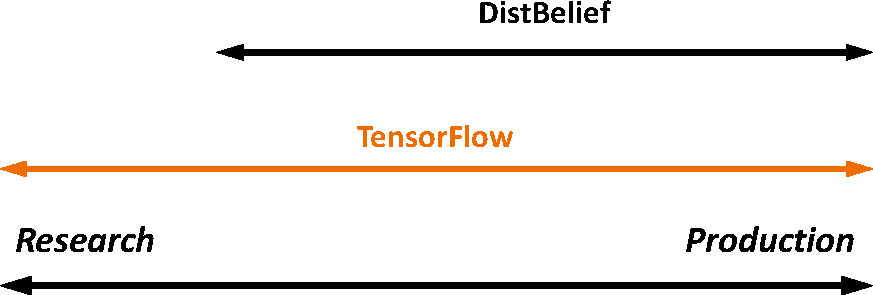
\includegraphics[width=.7\textwidth]{images/DistBeliefvsTensorFlow.pdf}\\
	\vspace{10pt} 
	\caption{Zielgruppenabdeckung von DistBelief und \gls{TF}~\cite{tf-sum17-keynote}}
	\label{fig:DBvsTF}
\end{figure}

\gls{TF} bietet zum einen genug Flexibilität für Forschungsprojekte, um mit neuen Modellen zu experimentieren, ist gleichzeitig aber hochperformant und robust, was beim Einsatz in Produktivsoftware wichtig ist. Modelle können somit also oft aus der Forschung direkt in Produktivumgebungen übernommen werden~\cite{tensorflow2016-whitepaper}.


\section{Hard- und Software Anforderungen}
Tensorflow wurde von Grund auf so gestaltet, dass es eine möglichst großen Bandbreite an Hardware zur Berechnung der \gls{NN} nutzen kann und auch größtenteils unabhängig von dem System ist, auf dem es ausgeführt wird.

\subsection{Betriebssysteme}
\gls{TF} ist seit dem Anfang auf Linux und MacOS lauffähig. Seit Version 0.12 wird außerdem Windows unterstützt~\cite{tf0.12}. Die reine Ausführung eines bereits trainierten Netzes (Inference) ist außerdem auch auf Android und iOS möglich~\cite{tensorflow2015-whitepaper}\cite{tensorflow2016-whitepaper}.

\subsection{Hardware Unterstützung}
Lernalgorithmen basieren oft auf aufwändigen Rechenoperationen, die zwar hoch parallelisierbar sind, meist jedoch auch große Abhängigkeiten beim Datenzugriff aufweisen. Ein Beispiel hierfür sind Matrix Multiplikationen. Mit dem Aufkommen von so genannten "`Generall Purpose GPUs"' die eine große Anzahl an Recheneinheiten und schnellen lokalen Speicher bieten, konnten \gls{NN} stark beschleunigt werden.

\gls{TF} bietet hier den Vorteil, dass es unabhängig von der vorhandenen Hardware eingesetzt werden kann. Es werden sowohl CPUs als auch eine Vielzahl von NVIDIA GPUs unterstützt. Im Moment können GPUs anderer Hersteller noch nicht genutzt werden, da gls{TF} die CUDA-API von NVIDIA nutzt. Diese "`CUDA Compute Capability"' muss von der Hardware auch mindestens in Version 3.0 unterstützt werden. Eine Liste mit allen unterstützen Karten kann auf der \href{https://developer.nvidia.com/cuda-gpus}{NVIDIA Homepage} gefunden werden~\cite{tfinstall}.

Neben diesen allgemein gehaltenen Recheneinheiten kann \gls{TF} auch spezielle Hardware für die Berechnungen nutzen. So gibt es von Google selbst sogenannte \glspl{TPU}, die eine enorme Beschleunigung von Inference ermöglichen und dabei vor allem wesentliche energieeffizienter sind, als CPUs oder auch GPUs~\cite{TPU}. Da es sich hierbei jedoch um proprietäre Hardware handelt, können diese \glspl{TPU} im Moment nur als Service in der Google Cloud genutzt werden~\cite{TPU2}. Außerdem kann der sogenannte "`Neural Compute Stick"' von Movidius (inzwischen Intel)~\cite{movidius} verwendet werden, der es auch auf leistungsschwacher Hardware wie zum Beispiel einem Raspberry Pi möglich macht, Inference von \gls{NN} durchzuführen.

In Tensorflow kann genau definiert werden, welche Schritte im Programmcode von welcher Recheneinheit ausgeführt werden sollen. So wird in Zeile zwei von \autoref{lst:tf-dev} angegeben, dass die dritte GPU im System verwendet werden soll\footnote{\gls{TF} beginnt bei null zu zählen}~\cite{tf-dev}.

\begin{minipage}{\linewidth}
\begin{lstlisting}[language=Python, label=lst:tf-dev, caption={Festlegung des Geräts, auf dem die Berechnung getätigt werden soll}]
# Creates a graph.
with tf.device('/device:GPU:2'):
  a = tf.constant([1.0, 2.0, 3.0, 4.0, 5.0, 6.0], shape=[2, 3], name='a')
  b = tf.constant([1.0, 2.0, 3.0, 4.0, 5.0, 6.0], shape=[3, 2], name='b')
  c = tf.matmul(a, b)
# Creates a session with log_device_placement set to True.
sess = tf.Session(config=tf.ConfigProto(log_device_placement=True))
# Runs the op.
print(sess.run(c))
\end{lstlisting}
\end{minipage}

In den Zeilen drei und vier werden zwei konstante Arrays definiert und in Zeile fünf wird die durchzuführende Rechenoperation festgelegt. In Zeile sieben wird eine TensorFlow Session erstellt und mit "`sess.run"' in Zeile neun wird schließlich die Berechnung angestoßen.

\subsection{Software Anforderungen}
\Gls{TF} ist sowohl für Python 2.7 verfügbar, als auch für Python 3 ab Version 3.4~\cite{tfinstall}. Alternativ sind aber auch Docker Images verfügbar.

Für die Verwendung von NVIDIA GPUs muss außerdem das CUDA® Toolkit in Version 8.0 	sowie cuDNN v6.0 installiert werden~\cite{tfinstall}.

\section{Softwarearchitektur von TensorFlow}
\Gls{TF} wurde als erweiterbare, plattformübergreifende Bibliothek konzipiert. \autoref{fig:architektur} zeigt, wie dies durch Modularisierung erreicht wurde. Dabei wird alles oberhalb der C-API als "`user-level"' bezeichnet und alles darunter als "`core library"'~\cite{tensorflow2016-whitepaper}.

\begin{figure}[htb!]
	\centering
	 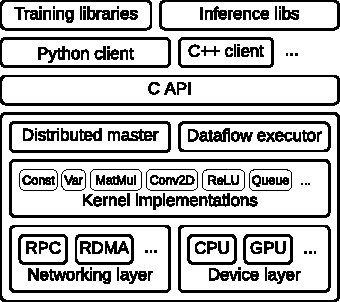
\includegraphics[width=.5\textwidth]{images/architektur.pdf}\\
	\vspace{10pt} 
	\caption{Die Architektur von \gls{TF}~\cite{tensorflow2016-whitepaper}}
	\label{fig:architektur}
\end{figure}

Die meisten Nutzer werden \gls{TF} über die bereitgestellten Client-Schnittstellen nutzen. Diese sind für die beiden Sprachen "`Python"' und "`C++"' vorhanden. Beide nutzen dabei eine C API, die den Zugriff auf die core-library von \gls{TF} ermöglicht. Diese wiederum wurden in C++ implementiert um Portabilität und Leistungsfähigkeit zu gewährleisten. Im user-level befinden sich außerdem noch Training- und Inference-Bibliotheken, in denen häufig genutzte Funktionen wie Backpropagation oder das Gradientenabstiegsverfahren aus
%%TODO ref!!
Kapitel 2.6 bereits implementiert wurden.

Der Kern von \gls{TF} besteht aus mehreren Komponenten. Der sogenannte "`distributed master"' teilt den Berechnungsgraphen in mehrere Sub-Graphen auf, die dann auf den einzelnen Recheneinheiten vom "`dataflow executor"' ausgeführt werden. Des weiteren sind mehr als 200 Standard-Operationen für zum Beispiel Array Manipulation oder Zustandsmanagement enthalten. Dabei wurde an vielen Stellen auf bereits bestehende Open-Source-Software aufgebaut, die eine effiziente Parallelberechnung auf Mehrkern-CPUs und GPUs sicherstellt.

Im "`Networking layer"' wurden erweiterte Netzwerkprotokolle wie "`gRPC over TCP"' oder "`RDMA over Converged Ethernet"' integriert, die eine schnelle Kommunikation zwischen entfernten Rechnern sicherstellen sollen. Doch auch innerhalb eines Rechners wurden zusätzliche Funktionen implementiert, die einen schnellen Datenaustausch von zum Beispiel zwei GPUs ermöglichen sollen.
\chapter{Der Allgemeine Workflow in TensorFlow}

Zu Beginn dieses Kapitels wird die Methodik der Aufteilung der Datensätze in Trainings-, Validierungs- und Testdaten erläutert, welches für die Beurteilung der Ergebnisse eines Modells unerlässlich ist. Anschließend erfolgt eine Einführung in das Visualisierungstool TensorBoard, mit dessen Hilfe sich die hier vorgestellten und noch weitere Vorgänge anschaulich abbilden lassen. Am Schluss werden noch die einzelnen Graphelemente näher betrachtet, wodurch sich umfangreiche Graphabbildungen erzeugen lassen. 
%\section{Die Tooling Pipeline}


\section{Vorgehensweise beim Trainingsprozess}


Eines der entscheidenden Kriterien über die Qualität des Modells ist die Prognose der Zielgröße auf zuvor ungesehenen Daten. Die Genauigkeit auf den Daten, mit denen das Modell trainiert wurde, geben keine grundlegende Aussage über die zu erwartende Genauigkeit auf zukünftige Daten. Deshalb ist es essentiell wichtig ungenutzte Testdaten zur Beurteilung mit einzubeziehen. Häufig müssen Entscheidungen über Metaparameter wie Neuronenanzahl, Stärke der Regularisierung, Art des Kernels getroffen werden. Daher unterteilt man die Datensätze in Trainings-, Validierungs- und Testdaten \cite{hoffmann2014proceedings}.
\vspace{10pt}

\begin{itemize} 
\item \textbf{Training} \vspace{5pt}

Trainingsdaten bilden die Grundlage für das überwachte Lernen. Hierbei werden durch eine Reihe von Beispielen Parameter wie die Gewichte der Verbindungen zwischen den Neuronen angepasst. Häufig besteht der Trainingsdatensatz aus Paaren von Eingangsvektoren und der dazugehörigen Antwortvektoren. \vspace{10pt}

\item \textbf{Validierung} \vspace{5pt}

Validierungsdaten dienen der Festlegung der optimalen Struktur des Modells, insbesondere zur Einstellung der optimalen Parameter des Lernalgorithmus wie die Lernrate oder die Anzahl der Trainingsepochen. Validierungsdatensätze werden auch für die Regularisierung von  \dq early stopping\grqq{} und bei der Zunahme des Fehlers im Validierungsdatensatz, da dies ein Zeichen für  \dq overfitting\grqq{} ist, angewandt. \vspace{10pt}

\item \textbf{Testen} \vspace{5pt}

Testdaten werden verwendet, um eine Bewertung eines endgültigen Modells zu ermöglichen, welche auf ungesehene Daten angewandt wurde.

\end{itemize}\vspace{10pt}


\textbf{Cross-Validation} \vspace{10pt}

Die Unterteilung des Datensatzes in einen festen Trainingssatz und einen festen Testsatz kann problematisch sein, wenn der Testsatz zu klein ist. Dies impliziert statistische Unsicherheit im Bereich des geschätzten Testfehlers. Abhilfe schafft die k-fache Kreuzvalidierung (Cross-Validation), welche die Daten in k disjunkte Teilmengen unterteilt, auf denen k Tests durchgeführt werden, wobei jeweils k-1 Teilmengen für das Training und die verbliebene Teilmenge zum Testen verwendet wird \cite{hoffmann2014proceedings}.

%https://books.google.de/books?id=93djocO3yVgC&hl=de&source=gbs_navlinks_s
%Proceedings. 22. Workshop Computational Intelligence, Dortmund, 6. - 7. Dezember 2012

\section{Die Visualisierung mit TensorBoard}

TensorBoard ist eine in TensorFlow enthaltene Webanwendung zur Visualisierung der Abläufe in einem neuronalen Netz. TensorBoard stellt eine Vielzahl an graphischen Elementen zur Verfügung, welche dem Entwickler vorallem das Debuggen oder die Optimierung eines erstellten Modells erleichtern. Ebenso können damit insbesondere komplexe Datenstrukturen zum besseren Verständnis anschaulich visualisiert werden. 

Bevor mit TensorBoard gearbeitet werden kann, muss nachfolgender Befehl in die Kommandozeile eingegeben werden:
\\

\begin{minipage}{\linewidth}
\begin{lstlisting}[language=bash, label={lst:tensorboard}]
C:\> tensorboard  --logdir=path/to/log_directory

\end{lstlisting}
\end{minipage}

\vspace{0.2cm}
wobei vorher im spezifizierten Log Ordner die gewünschten Event Daten mit der Klasse
\\

\begin{minipage}{\linewidth}
\begin{lstlisting}[language=Python, label={lst:FileWriter}]
tf.summary.FileWriter('path/to/log_directory')

\end{lstlisting}
\end{minipage}
\vspace{0.2cm}

abgespeichert werden müssen. Nachdem TensorBoard gestart wurde, navigiert man mit dem Browser zu folgender Seite:
\\

\begin{minipage}{\linewidth}
\begin{lstlisting}[language=Python, label={lst:localhost}]
http://localhost:6006

\end{lstlisting}
\end{minipage}
\vspace{0.2cm}

Falls keine Fehlermeldungen aufgetreten sind, sollte folgender Bildschirminhalt Abbildung \ref{fig:tensorboard_start} angezeigt werden. Um die Visualisierungen in den einzelnen Reiter zu erhalten, müssen diese vorher im Programm mit speziellen TensorFlow Klassen abgespeichert werden. In dem nachfolgenden Kapitel werden die einzelnen Reiter und der dazugehörigen Klasse vorgestellt. 
\\[1ex]

\begin{figure}[h!]
	\centering
	%\vspace{-35pt}
	%\hspace{-1.0cm} 
	 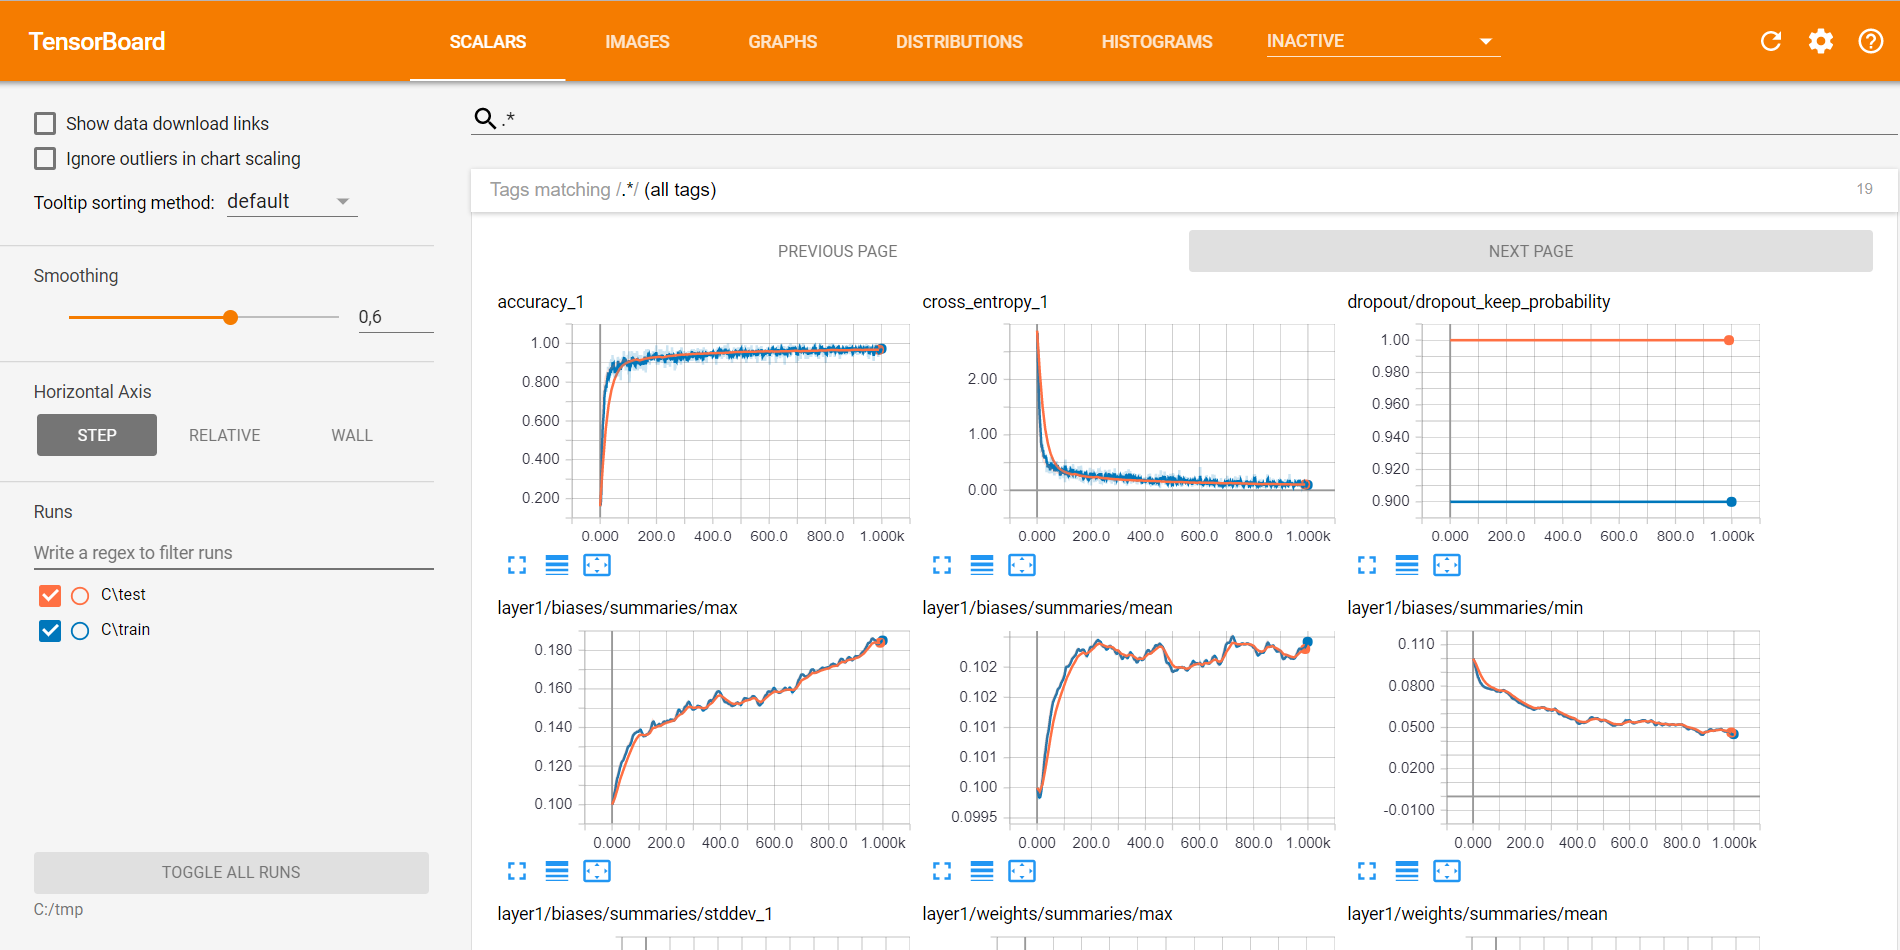
\includegraphics[width=1\textwidth]{images/Kapitel_3/TensorBoard_start.png}\\
	\vspace{10pt} 
	\caption[Die Startseite von TensorBoard]{Die Startseite von TensorBoard}
	\label{fig:tensorboard_start}
\end{figure}





\section{Die einzelnen Visualisierungsmöglichkeiten im Detail}

\subsection{Skalare}
%\textbf{\textit{Skalare}} 
\vspace{10pt}
Unter dem Reiter Skalare, welche mit der Klasse
\\

\begin{minipage}{\linewidth}
\begin{lstlisting} [label={lst:scalar}]
tf.summary.scalar(name, tensor, collections=None, family=None)
\end{lstlisting}
\end{minipage}

\vspace{0.2cm}

abgespeichert werden, können verschiedenste Statistiken während eines Trainingsprozesses visualisiert werden. Dies könnten zum Beispiel die Genauigkeit (Accuracy) oder Kreuzentropie (Cross Entropy) sein, welche in Abbildung \ref{fig:skalare} dargestellt sind. Hierbei wird die Genauigkeit über den einzelnen Trainingsschritten aufgetragen. Wählt man mit der Maus einen bestimmten Datenpunkt aus, so werden zahlreiche weitere Informationen angezeigt. Ebenso ist hierbei ersichtlich, dass auch Trainings- und Testdaten gleichzeitig angezeigt und miteinander verglichen werden können \cite{tensorboard.2017}.

\vspace{0.3cm}
\begin{figure}[h!]
	\centering
	%\vspace{-35pt}
	%\hspace{-1.0cm} 
	 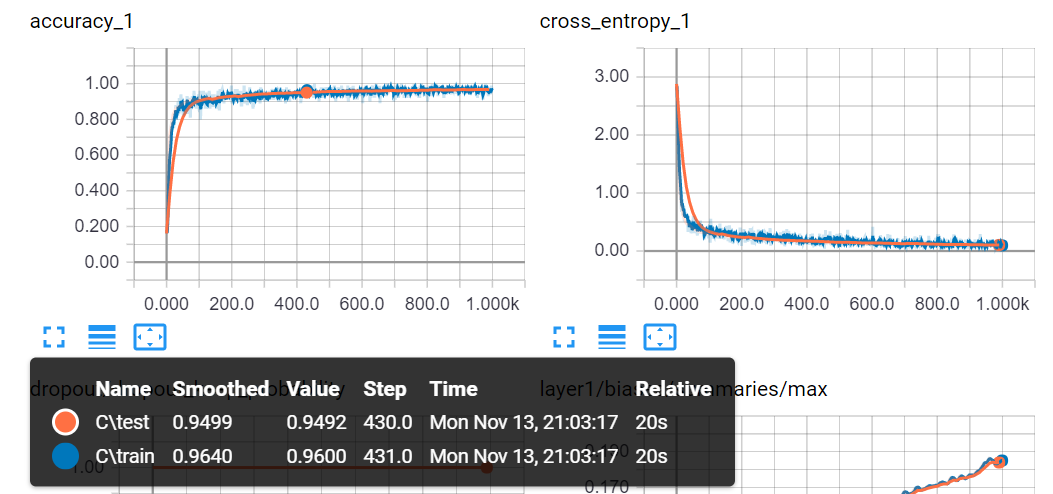
\includegraphics[width=0.8\textwidth]{images/Kapitel_3/skalars.png}\\
	\vspace{10pt} 
	\caption[Visualisierung der 'Accuracy' und 'Cross\_entropy' über die einzelnen Trainingsschritte]{Visualisierung der 'Accuracy' und 'Cross\_entropy' über die einzelnen Trainingschritte}
	\label{fig:skalare}
\end{figure}





\subsection{Bilder}
%\textbf{\textit{Bilder}}
%\vspace{30pt}

Innerhalb des Reiters Bilder, welche mit der Klasse

\vspace{0.6cm}
\begin{minipage}{\linewidth}
\begin{lstlisting} [label={lst:image}]
tf.summary.image(name, tensor, max_outputs=3, collections=None, family=None)
\end{lstlisting}
\end{minipage}
\vspace{0.3cm}

\begin{figure}[htb!]
	\centering
     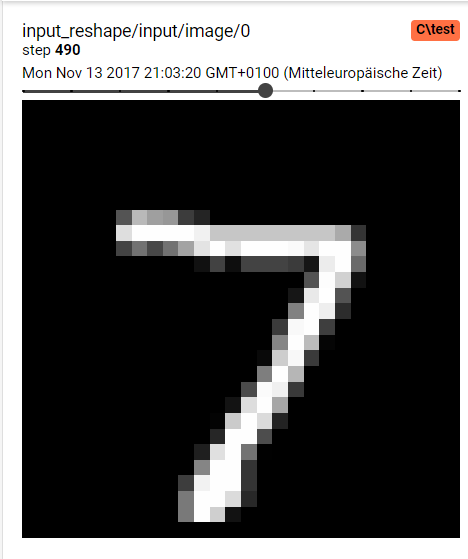
\includegraphics[width=6cm]{images/Kapitel_3/images.png}
	\vspace{10pt} 
	\caption{Bild des Testschrittes 490}
	\label{fig:TensorBoard_image}
\end{figure}

abgespeichert werden, können zur genaueren Analyse die Test- und Trainingsbilder eingesehen werden. Wie in Abbildung \ref{fig:TensorBoard_image} ersichtlich, ist über den Bildern eine Scrollbar vorhanden mit dieser können einzelne Test- und Trainingsschritte ausgewählt werden, wodurch genau ersichtlich wird, welches Bild zum aktuellen Durchlauf gehört \cite{tensorboard.2017}.
\vspace{50pt}
\newpage


\begin{figure}[t]
\begin{minipage}[t]{0.475\textwidth}
\centering
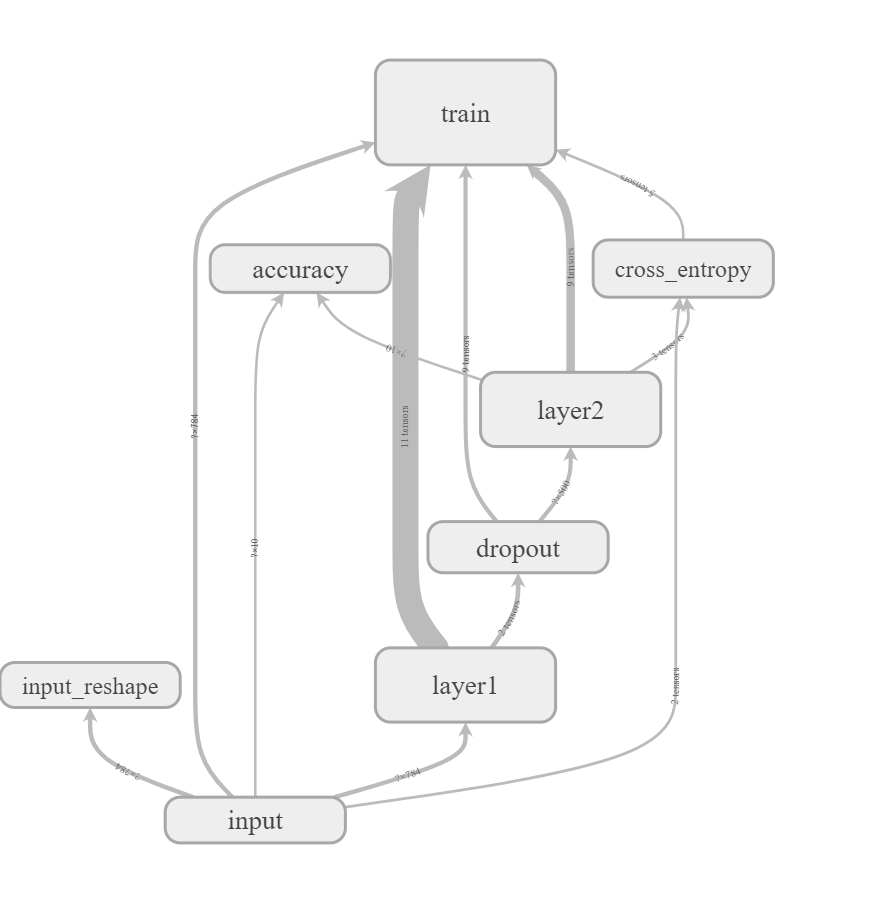
\includegraphics[width=0.9\textwidth]{images/Kapitel_3/graph.png}
\caption{TensorFlow Graph mit definierten Name scopes}
\label{fig:TensorFlow_Graph}
\end{minipage}
\hfill
\begin{minipage}[t]{0.475\textwidth}
\centering
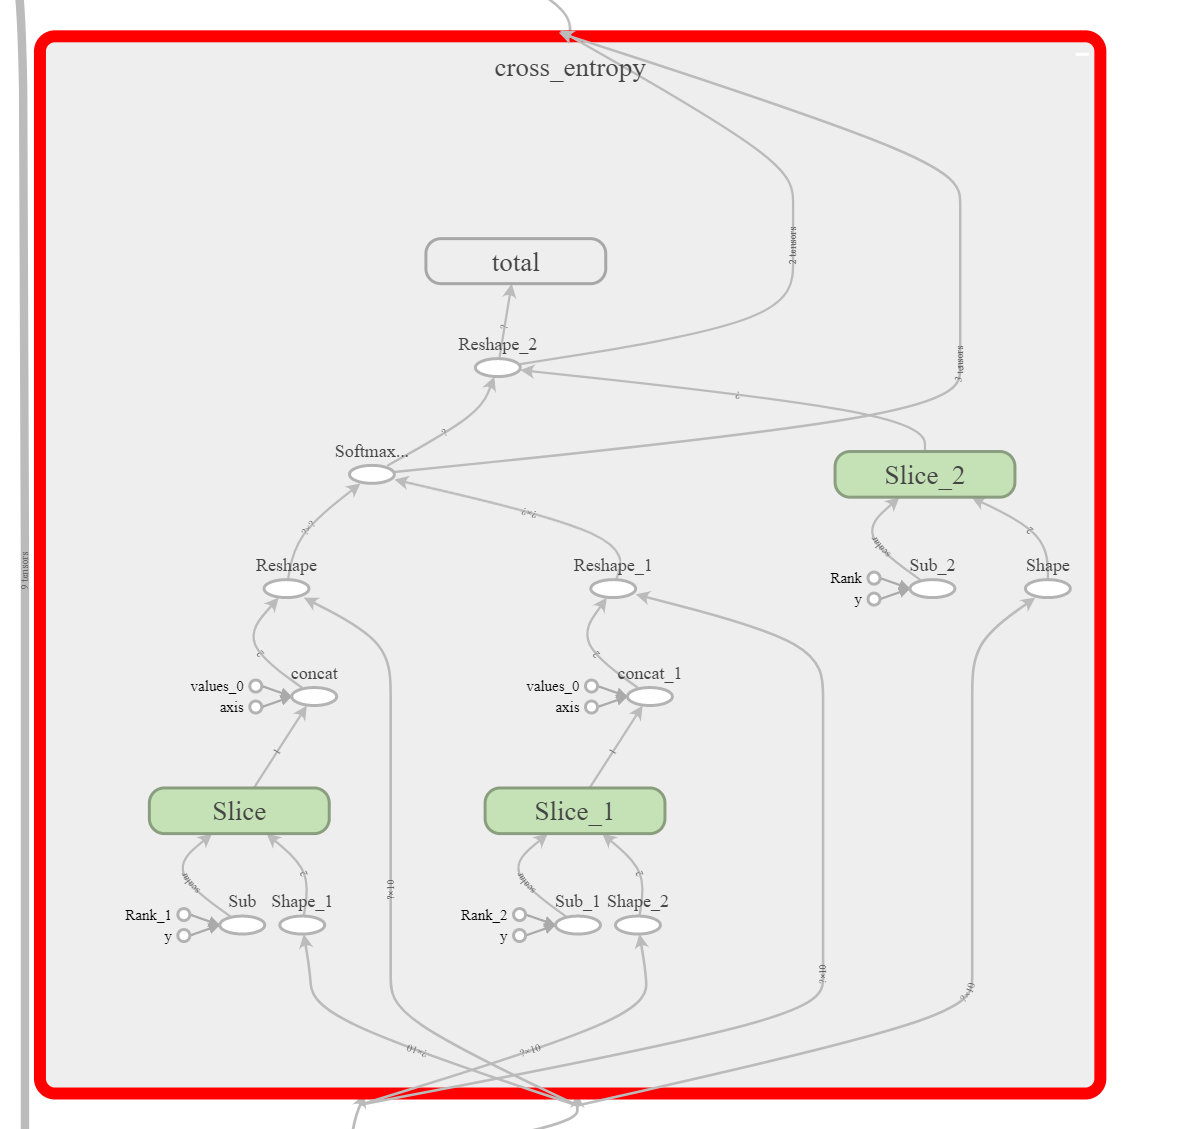
\includegraphics[width=0.9\textwidth]{images/Kapitel_3/graph1.png}
\caption{Name scope 'cross\_entropy' unterteilt in weiteren Operationen}
\label{fig:name_scope_cross_entropy}
\end{minipage}
\end{figure}



\subsection{Graphen} \label{sub:tb-graph}
%\textbf{\textit{Graphen}}
\vspace{10pt}
Unter dem Reiter Graphen befindet sich das komplette TensorFlow Model als Graph,  wie in Abbildung \ref{fig:TensorFlow_Graph} zu sehen ist. Nur wenn im vorher erstellten Programm Name scopes zu den gewünschten Operationen definiert wurden, werden diese in TensorBoard als Graph angezeigt. Mit nachfolgendem Befehl in Zeile 1 erhält man einen \textit{cross\_entropy} Name scope: 
\\

\begin{minipage}{\linewidth}
\begin{lstlisting} [label={lst:graph}]
with tf.name_scope('cross_entropy'):
  diff = tf.nn.softmax_cross_entropy_with_logits(targets=y_, logits=y)
  with tf.name_scope('total'):
    cross_entropy = tf.reduce_mean(diff)
tf.summary.scalar('cross_entropy', cross_entropy)
\end{lstlisting}
\end{minipage}
\vspace{0.2cm}

Der Name scope \textit{cross\_entropy} in Abbildung \ref{fig:name_scope_cross_entropy} kann natürlich wiederum in mehrere Untergruppierungen aufgeteilt werden. So erhält man eine übersichtliche Visualisierung komplexer TensorFlow Modelle \cite{tensorboard.2017}.






\subsection{Histogramme}
%\textbf{\textit{Histogramme}}
\vspace{10pt}
Unter dem Reiter Histogramme, welche mit der Klasse
\\

\begin{minipage}{\linewidth}
\begin{lstlisting} [label={lst:histogram}]
tf.summary.histogram(name, values, collections=None, familiy=None)
\end{lstlisting}
\end{minipage}
\vspace{0.2cm}


abgespeichert werden, wird die statistische Verteilung eines Tensors über der Zeit dargestellt. Im Histogramm sind zeitliche \dq Slices\grqq{} der Daten visualisiert, wobei jeder einzelne Slice ein Histogramm des Tensors in einem einzelnen Schritt darstellt. In Abbildung \ref{fig:histogram} ist ein einzelner Slice schwarz markiert \cite{tensorboard.2017}.

\vspace{0.6cm}
\begin{figure}[h!]
	\centering
	%\vspace{-35pt}
	%\hspace{-1.0cm} 
	 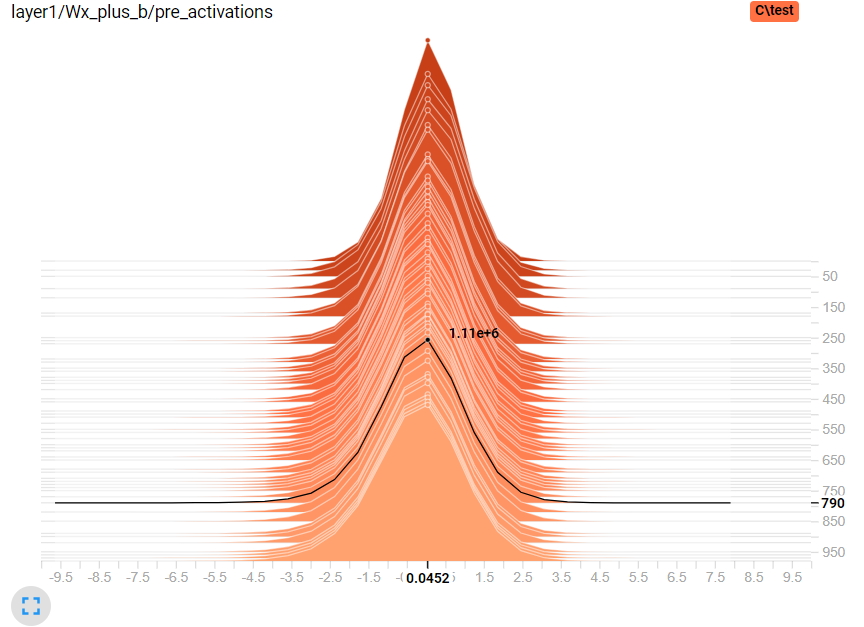
\includegraphics[width=0.7\textwidth]{images/Kapitel_3/histogram.png}\\
	\vspace{10pt} 
	\caption[Visualisierung eines Histogramms über die einzelnen Trainingsschritte]{Visualisierung eines Histogramms über die einzelnen Trainingschritte}
	\label{fig:histogram}
\end{figure}






\subsection{Verteilungen}
%\textbf{\textit{Verteilungen}}
\vspace{10pt}

Unter dem Reiter Verteilungen, welche ebenfalls mit der Klasse
\\

\begin{minipage}{\linewidth}
\begin{lstlisting} [label={lst:distribution}]
tf.summary.histogram(name, values, collections=None, familiy=None)
\end{lstlisting}
\end{minipage}
\vspace{0.2cm}

abgespeichert werden, befindet sich eine weitere Möglichkeit der Visualisierung der statistischen Verteilung. Hierbei repräsentiert die oberste Linie den über die Zeit veränderten maximalen Wert, die unterste Linie den minimalen Wert und die mittlere Linie den veränderten Median über der Zeit \cite{tensorboard.2017}.

\vspace{0.4cm}
\begin{figure}[h!]
	\centering
	%\vspace{-35pt}
	%\hspace{-1.0cm} 
	 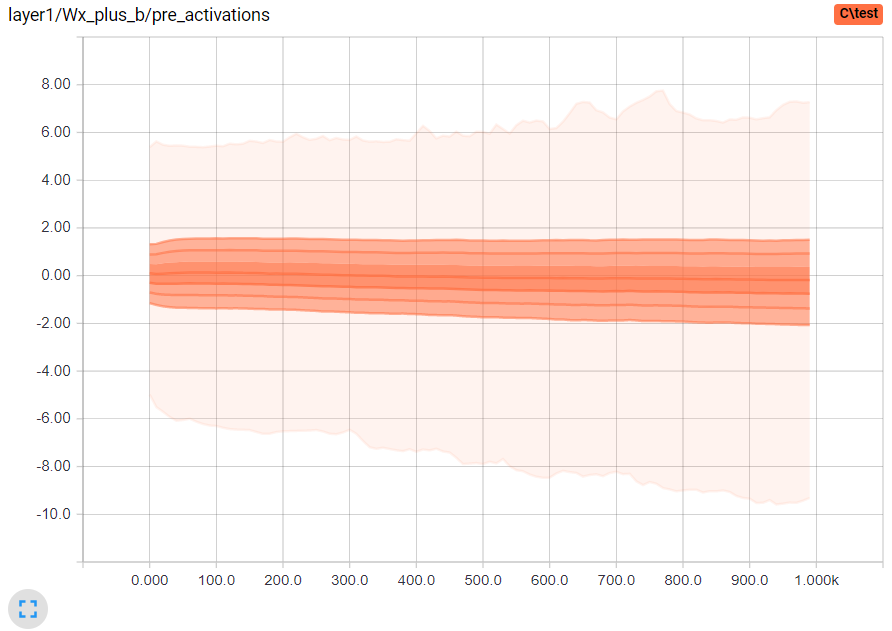
\includegraphics[width=0.8\textwidth]{images/Kapitel_3/distribution.png}\\
	\vspace{10pt} 
	\caption[Eine weitere Möglichkeit der Visualisierung der statistischen Verteilung]{Eine weitere Möglichkeit der Visualisierung der statistischen Verteilung}
	\label{fig:verteilung}
\end{figure}

%\vspace{0.3cm}



\subsection{Projektor}

%\textbf{\textit{Projektor}}

Die Auswahl des Reiters Projektors ermöglicht die höherdimensionale Visualisierung der Eingabedaten. Nachfolgend eine mögliche Konfiguration des Projektors:
\vspace{0.1cm}
\\

\begin{minipage}{\linewidth}
\begin{lstlisting} [label={lst:embedding}, caption={Konfiguration eines Projektors in TensorFlow \cite{embedding_viz}}]
from tensorflow.contrib.tensorboard.plugins import projector

# Use the same LOG_DIR where you stored your checkpoint.
summary_writer = tf.train.SummaryWriter(LOG_DIR)

# Format: tensorflow/contrib/tensorboard/plugins/projector/projector_config.proto
config = projector.ProjectorConfig()

# You can add multiple embeddings. Here we add only one.
embedding = config.embeddings.add()
embedding.tensor_name = embedding_var.name

# Link this tensor to its metadata file (e.g. labels).
embedding.metadata_path = os.path.join(LOG_DIR, 'metadata.tsv')

# Saves a configuration file that TensorBoard will read during startup.
projector.visualize_embeddings(summary_writer, config)
\end{lstlisting}
\end{minipage}
\vspace{0.3cm}

Hierbei werden zwei wesentliche Darstellungen unterschieden.
\vspace{10pt}

\begin{itemize} 
\item \gls{PCA} \vspace{10pt}

Ein häufiges Problem bei multivariaten Daten ist, dass diese nicht im zweidimensionalem Raum dargestellt werden können.  Hierbei werden bei der Hauptkomponentenanalyse (PCA) die Daten so auf eine zweidimensionale (bzw. dreidimensionaler) Ebene projiziert, mit der Erwartung, dass diese neue Darstellung eventuell vorhandenes Rauschen herausfiltert und versteckte Strukturen zum Vorschein bringt \cite{pca}.
%http://www.statistics4u.info/fundstat_germ/cc_pca.html
\begin{figure}[h!]
	\centering
	%\vspace{-35pt}
	%\hspace{-1.0cm} 
	 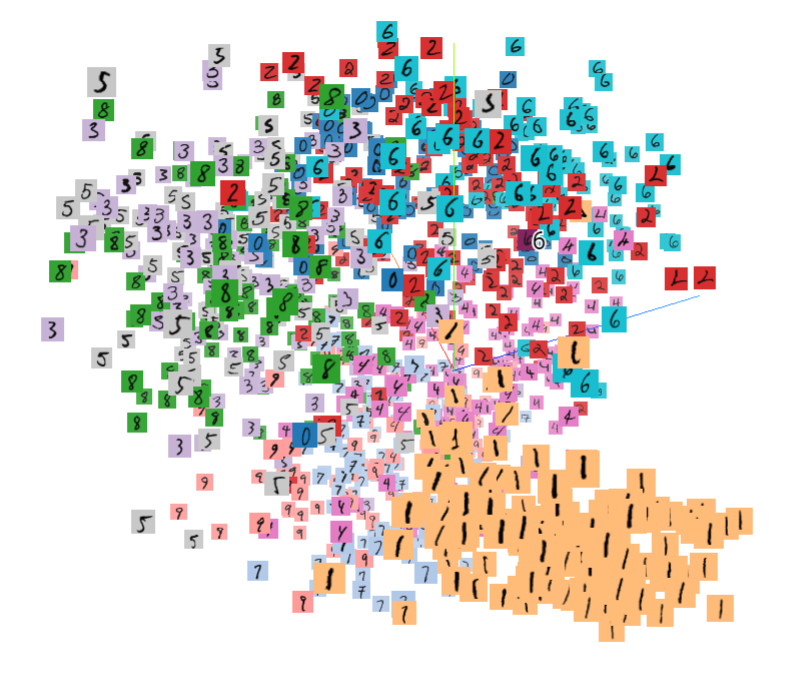
\includegraphics[width=0.8\textwidth]{images/Kapitel_3/projektor_pca.png}\\
	\vspace{10pt} 
	\caption[Visualisierung der PCA]{Visualisierung der PCA} \vspace{0.7cm}
	\label{fig:pca}
\end{figure}



\item \gls{t-SNE} \vspace{10pt}

Diese Technik der Dimensionsreduktion eignet sich besonders gut, um hochdimensionale Daten in einen Raum von zwei oder drei Dimensionen zu projizieren. Hierbei wird jedes hochdimensionale Objekt durch einen zwei- oder dreidimensionalen Punkt modelliert, sodass ähnliche Objekte durch nahe gelegene Punkte und ungleiche Objekte durch entfernte Punkte modelliert werden \cite{t-sne}.


\begin{figure}[h!]
	\centering
	%\vspace{-35pt}
	%\hspace{-1.0cm} 
	 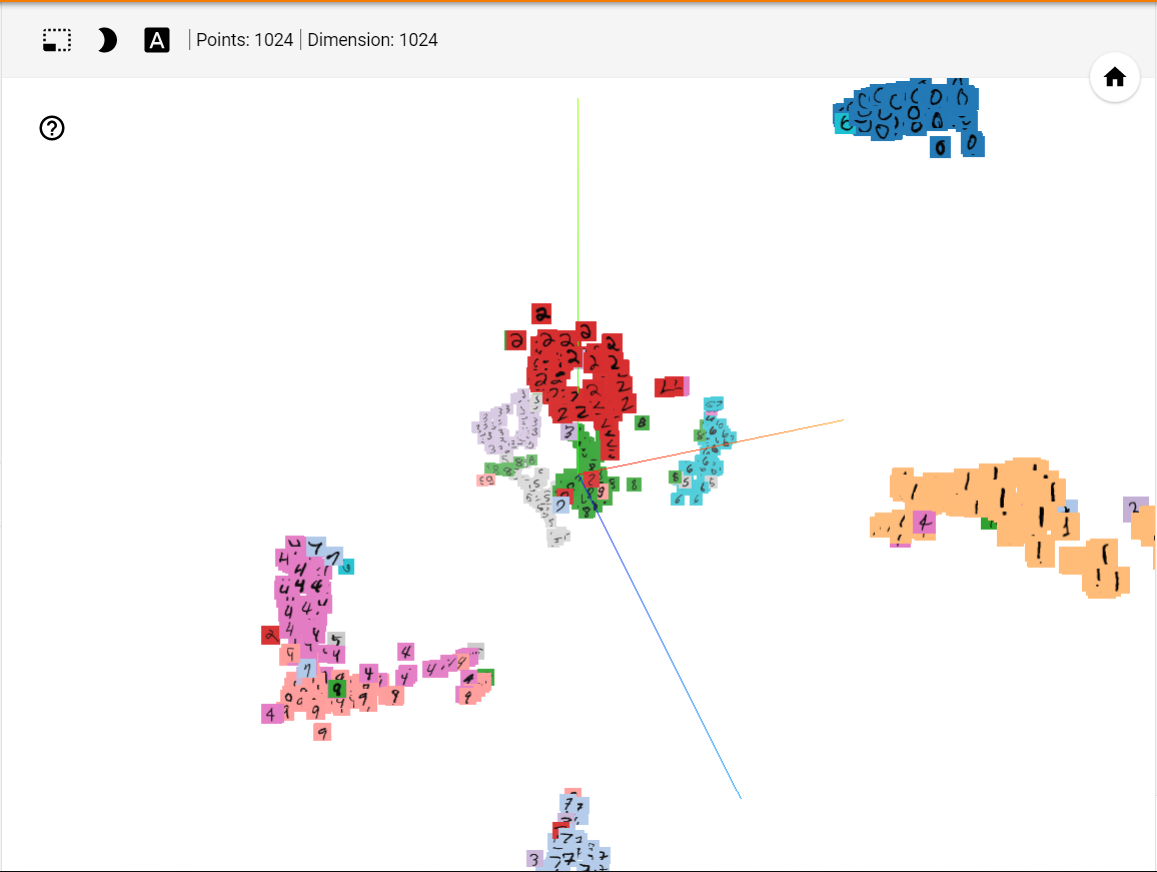
\includegraphics[width=0.8\textwidth]{images/Kapitel_3/projektor_t-sne.png}\\
	\vspace{15pt} 
	\caption[Visualisierung der t-SNE]{Visualisierung der t-SNE}
	\label{fig:t-sne}
\end{figure}

\end{itemize}


\subsection{Audio und Text}

Unter dem Reiter Audio können mit der Klasse
\\

\begin{minipage}{\linewidth}
\begin{lstlisting} [label={lst:audio}]
tf.summary.audio(name, tensor, sample_rate, max_outputs=3, collections=None, family=None)
\end{lstlisting}
\end{minipage}
\vspace{0.2cm}

abspielbare Audio-Widgets eingebettet werden.\\

Ebenso können unter dem Reiter Text mit der Klasse
\\

\begin{minipage}{\linewidth}
\begin{lstlisting} [label={lst:text}]
tf.summary.text(name, tensor, collections=None)
\end{lstlisting}
\end{minipage}
\vspace{0.2cm}

Textausschnitte abgespeichert werden. Zusätzliche Funktionen wie Hyperlinks, Listen und Tabellen werden unterstützt \cite{tensorboard.2017}.





\newpage

\section{Die Graphelemente im Datenfluss}

 Dafür wurden zahlreiche unterschiedliche Elemente definiert, welche nachfolgend kurz erläutert werden \cite{graph_viz}.
\\

\begin{tabular}{ p{4cm}p{10.8cm} ll }

\textbf{Namespace} \tabularnewline 
\includegraphics[width=0.1\textwidth]{images/Kapitel_3/namespace.png}
\label{fig:namespace}
 & High-level Knoten repräsentiert einen definierten Namensbereich.   \tabularnewline
  
\textbf{Unconnected series} \tabularnewline 

\includegraphics[width=0.1\textwidth]{images/Kapitel_3/Unconnected_series.png}
\label{fig:Unconnected_series}
 & Nummerierte Knoten, die nicht miteinander verbunden sind. \tabularnewline
  
\textbf{Connected series} \tabularnewline 

\includegraphics[width=0.1\textwidth]{images/Kapitel_3/Connected_series.png}
\label{fig:Connected_series}
 & Nummerierte Knoten, die miteinander verbunden sind. \tabularnewline 
 
\textbf{Operation node} \tabularnewline 

\includegraphics[width=0.1\textwidth]{images/Kapitel_3/Operation_node.png}
\label{fig:Operation_node}
 & Ein Knoten der eine einzelne Operation darstellt.  \tabularnewline 
 
\textbf{Constant} \tabularnewline 

\includegraphics[width=0.08\textwidth]{images/Kapitel_3/Constant.png}
\label{fig:Constant}
 & Repräsentiert eine Konstante im Programm.  \tabularnewline 

\textbf{Summary node} \tabularnewline 

\includegraphics[width=0.07\textwidth]{images/Kapitel_3/Summary_node.png}
\label{fig:Summary_node}
 & Dieser Knoten stellt eine Zusammenfassung dar.  \tabularnewline 

\textbf{Dataflow edge} \tabularnewline 

\includegraphics[width=0.1\textwidth]{images/Kapitel_3/Dataflow_edge.png}
\label{fig:Dataflow_edge}
 & Durchgezogener Pfeil zeigt den Datenfluss zwischen den Operationen an.  \tabularnewline
 
\textbf{Control edge} \tabularnewline 

\includegraphics[width=0.1\textwidth]{images/Kapitel_3/Control_dependency_edge.png}
\label{fig:Control_dependendy_edge}
 & Gepunkteter Pfeil zeigt die Steuerungsabhängigkeit zwischen den Operationen an.  \tabularnewline 
 
\textbf{Reference edge} \tabularnewline 

\includegraphics[width=0.1\textwidth]{images/Kapitel_3/Reference_edge.png}
\label{fig:Reference_edge}
 & Gelber Pfeil bedeutet, dass die ausgehende Operation die ankommende mutieren kann   \tabularnewline 
% & \tabularnewline
\end{tabular}
\\

\chapter{Ausblick}


%\section{}

%\section{}


%\input{Kapitel/5_chapter}

\clearpage
\phantomsection

%\selectlanguage{american}%
\selectlanguage{ngerman}
\addcontentsline{toc}{chapter}{Abbildungsverzeichnis}
\listoffigures
\newpage{}

\clearpage
\phantomsection

\addcontentsline{toc}{chapter}{Tabellenverzeichnis}
\listoftables
\newpage{}

\clearpage
\phantomsection


\addchap{Anhang}




\newpage{}

\clearpage
\phantomsection

\bibliographystyle{bibtex-daten/unsrtdin}
\addcontentsline{toc}{chapter}{\bibname}\nocite{*}
\bibliography{bibtex-daten/wissenschaftliches_seminar}

\end{document}
